% The "%" character denotes a comment
\documentclass[prb,preprint]{revtex4-1}
\usepackage{amsmath}  % needed for \tfrac, \bmatrix, etc.
\usepackage{amsfonts} % needed for bold Greek, Fraktur, and blackboard bold
\usepackage{graphicx} % needed for figures

\begin{document}
\title{PHYS 333 Project Proposal}
\author{Adam Stammer}
%\email{adam.stammer@go.winona.edu}

\date{\today}

%if you include an abstract, it goes here
\begin{abstract}
For my final project in PHYS-333 Microcontrollers class in the spring of 2020, I propose the design and building of a laser harp. This devices can be described as an electronic instrument controlled by blocking and unblocking laser beams to create a digital audio output. They look super cool in the dark with a fog machine. As of now the options for commercial laser harps are limited and not very standardized. Designing my own I hope to not only customize it to my own needs, but keep the cost as low as possible.
\end{abstract}

\maketitle
%title page ends here




\section{Goals}
The laser harp would be small and portable, lightweight, and cost effective. It needs to produce an audio output based on light reflections from a laser beam. This beam will be split into multiple beams, such that each beam is registered as a different output frequency. These will likely be stepped like the keys of a piano, but could be customized to fit particular needs. The output will ideally be a Midi port allowing far more control of the output but could go direct to a speaker output. This should all be packaged in a format no larger than an oscilloscope.

\section{Design Questions}
\subsection{Stepper Motor}
Stepper motors can be 4 or 6 wire controlled, each handled different. They can also have varying power levels, speeds, and torque. Size is also a consideration, as is the step resolution angle. Each of these features will change the design so I need to figure out what kind of stepper motor to use. Higher power motors may also require external power supplying circuits as to not fry the arduino.

\subsection{Microcontroller}
In the pursuit of keeping costs low I'd like to use the simples microcontroller possible. I'm considering an arduino nano, but I'm also considering using the ATMega chip that runs the Arduino Uno, but as a barebones mcirochip. I'll have to determine the microcontroller requirements before I can make that call.

\subsection{Laser Emitter}
There's a lot of laws regarding laser emitter strength which I may have to be careful of. I also need to research the reflection/brightness/detection characteristics of various laser colors and find a photodetector to match.

\subsection{MIDI}
I have next to no idea how MIDI works from a hardware standpoint, so that will require a good bit of research.

\subsection{Encasing}
I'm thinking about 3d printing a case to put it in but that's kind of a last step thing so I'm not too worried about it right now.

\section{Initial Hardware Requirements}
I plan on buying my own components for this project so that I can keep it, and because much of what I need is not available in the lab. As such this is a very rough component list.

\vspace{10mm}

Stepper Motor, Arduino, Resistors, Midi Jack, Laser Diode, Mirror, Case/Stand, Laser Detector, (Probably) H-bridge, power supply


\section{Further Reading}
I got this idea a few years ago from \url{}. I'm trying to design this entirely on my own but this will be a backup resource if I get lost or stuck. It should give a clearer idea of what my goals are.

\pagebreak

\section{(Very) Rough Design Sketch}
\begin{figure}[ht]
	\centering
	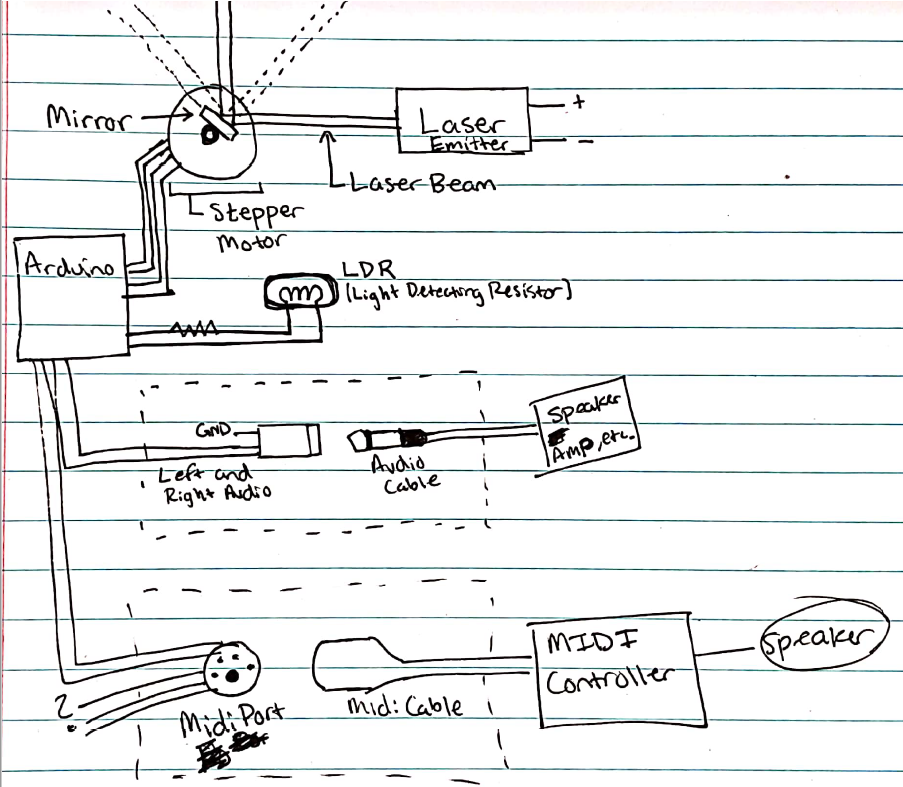
\includegraphics[width=5.75in]{design.png}
	\caption{Proposal Design Sketch}
	\label{fig1}
\end{figure}

\end{document}
